%!TEX root = ../thesis.tex
%*******************************************************************************
%****************************** Second Chapter *********************************
%*******************************************************************************

\chapter{Reconstruction}
\label{sec:SimReco_Reco}

Before it is used in the measurement of a physics process such as \ttbar production, the data taken by the detector needs to be reconstructed.
This reconstruction is performed offline, opposed to the online reconstruction for the trigger system.
The purpose of the reconstruction is to identify particles or groups of particles like jets, together called physics objects, and measure their properties.
Kinematic properties like the \pt and $\eta$ of a particle are the basic parameters of interest, but the reconstruction also includes other features like the charge or the isolation of particles.

Following a general introduction, this chapter describes the reconstruction for the different objects starting with tracks and vertices in Section \ref{sec:SimReco_Track}.
The reconstruction of electrons is described in Section \ref{sec:SimReco_Ele}.
The reconstruction of muons is described in Section \ref{sec:SimReco_Mu}.
The reconstruction of jets is described in Section \ref{sec:SimReco_jetReco}, while Section \ref{sec:SimReco_BjetReco} describes the identification of jets originating from a b quark.

As illustrated in Figure \ref{fig:reco_pflow}, different particles deposit energy in different parts of the detector.
The tracks of charged particles are bent by the magnetic field, while neutral particles are unaffected.
Similarly, only charged particles leave a signal in the tracker, as particles without a charge do not ionize the tracker material.
Electrons and photons deposit the main amount of their energy in the ECAL, whereas neutral and charged hadrons mainly deposit energy in the HCAL.
Muons are mainly detected by muon system in the outermost parts of the detector and in the inner tracker.

\begin{figure}[htbp!]
  \begin{center}
      \resizebox{0.80 \textwidth}{!}{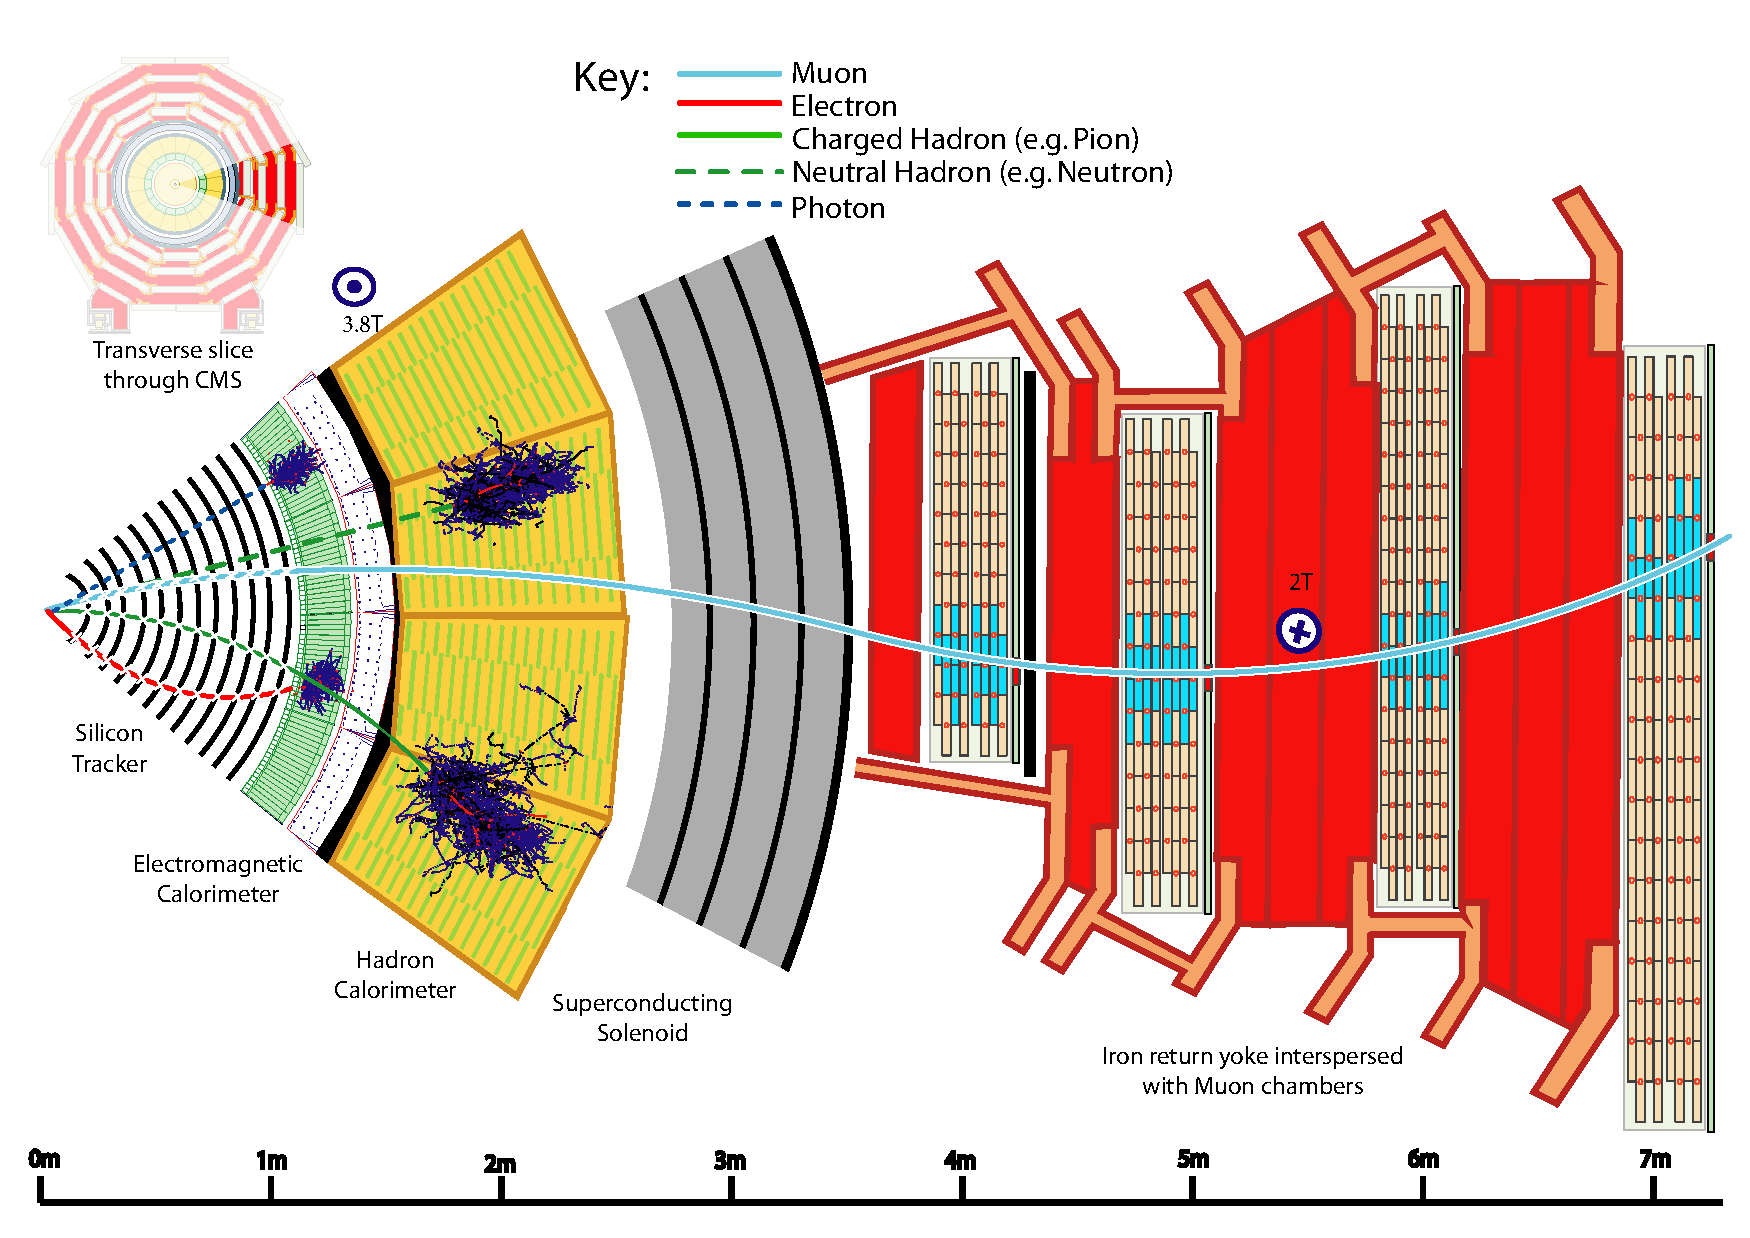
\includegraphics{SimReco/Figures/ParticleFlow.pdf}}
\caption{Illustration of the interaction of specific particles in a transverse slice of the CMS detector \cite{Sirunyan:2017ulk}.
  \label{fig:reco_pflow}}
  \end{center}
\end{figure}

Physics objects are reconstructed by combining the information from all parts of the detector using the Particle Flow algorithm \cite{Sirunyan:2017ulk}.
The tracks from the tracker and the muon system and the clusters from the calorimeters are combined to identify each final state particle.
This includes charged and neutral hadrons within jets. The Particle Flow algorithm allows for a more precise measurement of the energy and (for charged particles) the direction of particles.
It also allows to calibrate and to validate the different parts of the detector. All reconstruction methods described in this chapter are based on Particle Flow techniques.

In general, the probability to correctly reconstruct a particle can be different in simulation and measured data. Typically, these differences are small, since the detector response
is modelled and the reconstruction algorithms for data and simulation are the same. Nevertheless, small differences remain, which are corrected in simulated events.
These corrections are typically defined separately for each physics object by measuring the reconstruction efficiency independently in simulation and measured data.
The simulation is then corrected to fit the efficiency measured in data. Resolution effects are corrected in a similar manner.

\section{Tracking and vertex reconstruction}
\label{sec:SimReco_Track}


The aim of the tracking algorithm is to provide the properties of charged particles, for example the origin, the transverse momentum and the direction \cite{Sirunyan:2017ulk}.
The CMS track reconstruction itself is based on Kalman-Filtering \cite{Adam:934067} and consists of three steps starting with a seed of a few hits consistent with the trajectory of a charged particle.
The subsequent steps are the collection of hits from all tracker layers along the trajectory and the fitting to precisely determine the kinematic properties of the particle.
The tracking efficiency can be increased by repeating the track finding with different conditions \cite{1748-0221-9-10-P10009}, such as the quality requirement of the initial seed or the result of the fit.

The gain in efficiency through iterative tracking is presented in Figure \ref{fig:reco_trackingEff} showing the efficiency and the misreconstruction rate for tracks depending on the \pt of the charged particle for 
multiple different tracking algorithms. The efficiency is determined from simulation where tracks are considered to be reconstructed correctly if they can be associated to a simulated particle. Correspondingly, 
misreconstructed tracks cannot be associated to a simulated particle. 
Including all iterations shows the highest efficiency and a comparative mistag rate. In general, the efficiency decreases dramatically for high \pt tracks (see Section \ref{set:det_tracker}), especially for tracks with $\pt > 100 \gev$.
As shown in Figure \ref{fig:reco_trackingEff}, the misreconstruction rate increases with higher \pt, but the effect can be mitigated when the rest of the detector is taken into account.

\begin{figure}[htbp!]
  \begin{center}
      \resizebox{0.49 \textwidth}{!}{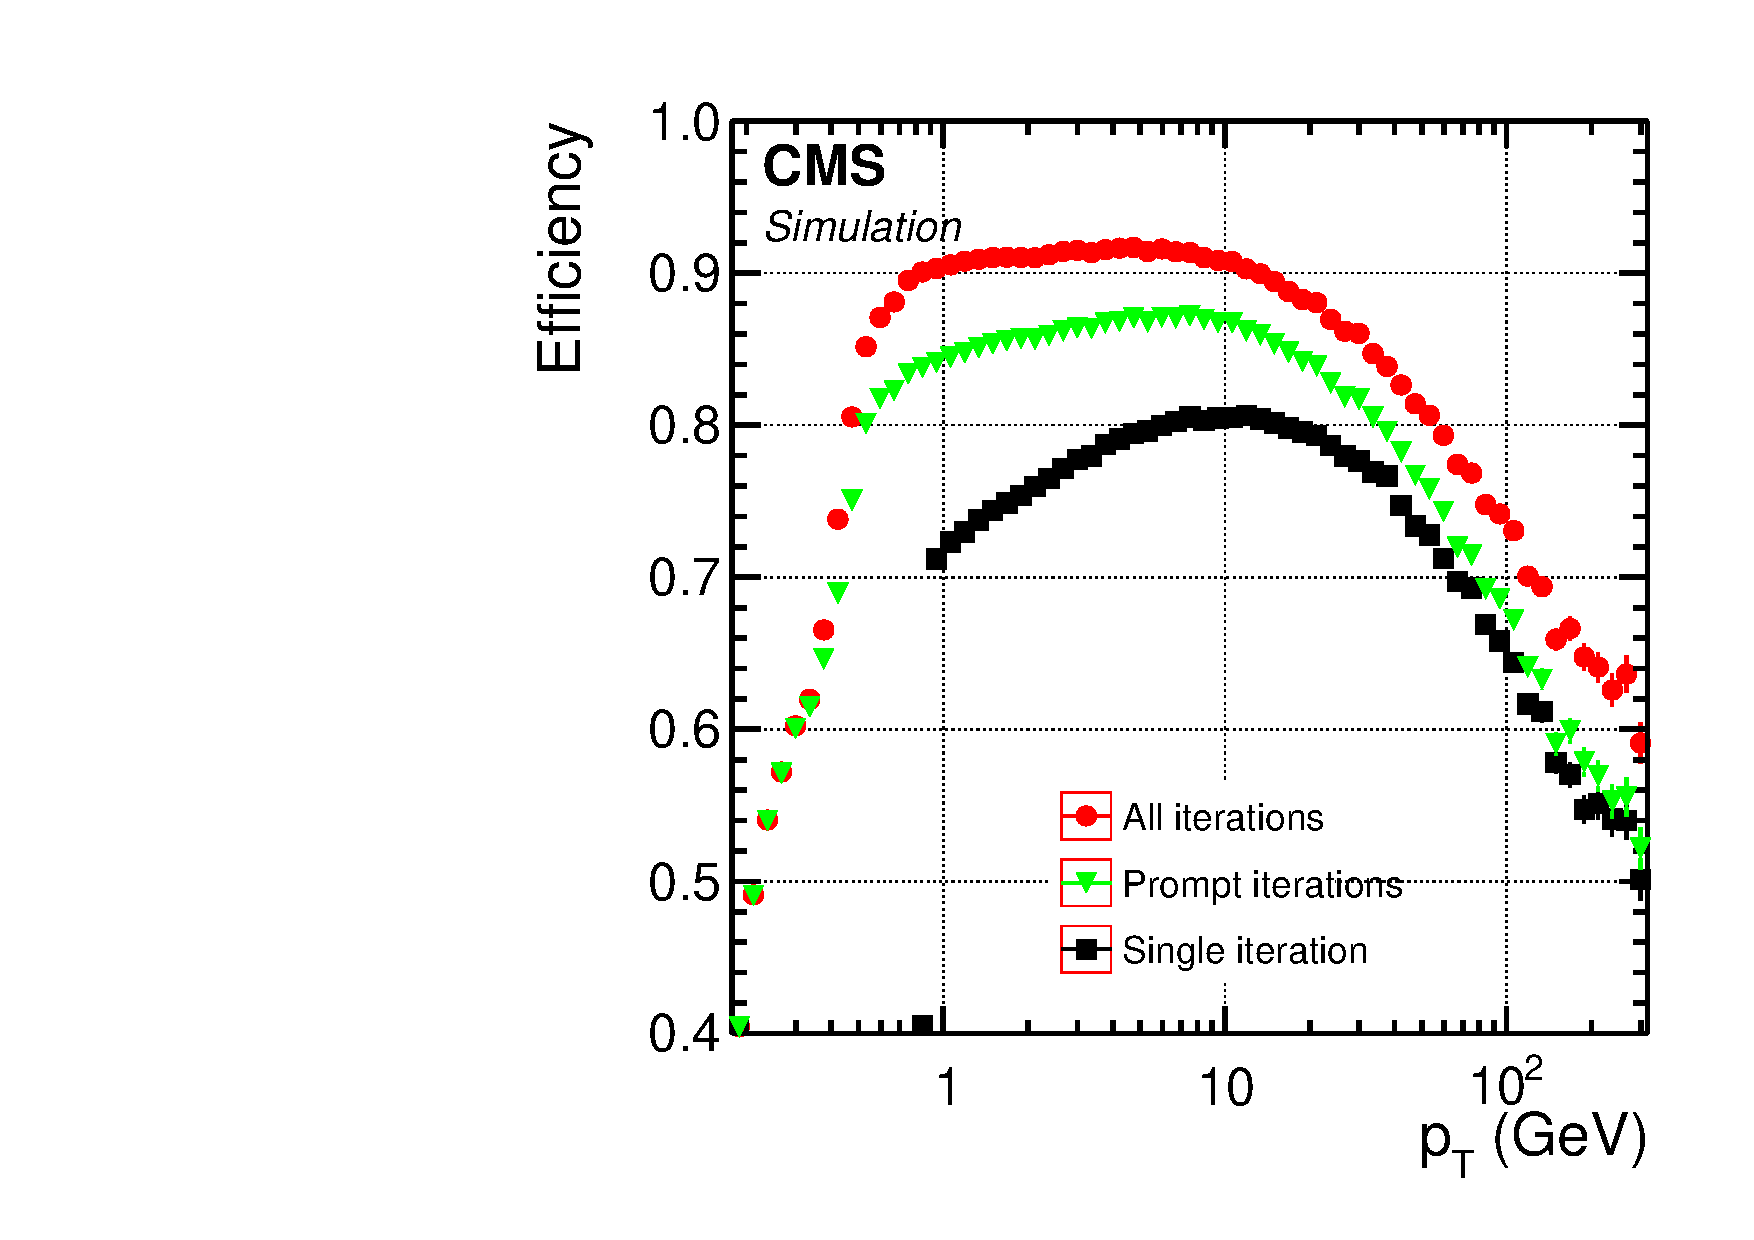
\includegraphics{SimReco/Figures/TrackingEff.pdf}}
      \resizebox{0.49 \textwidth}{!}{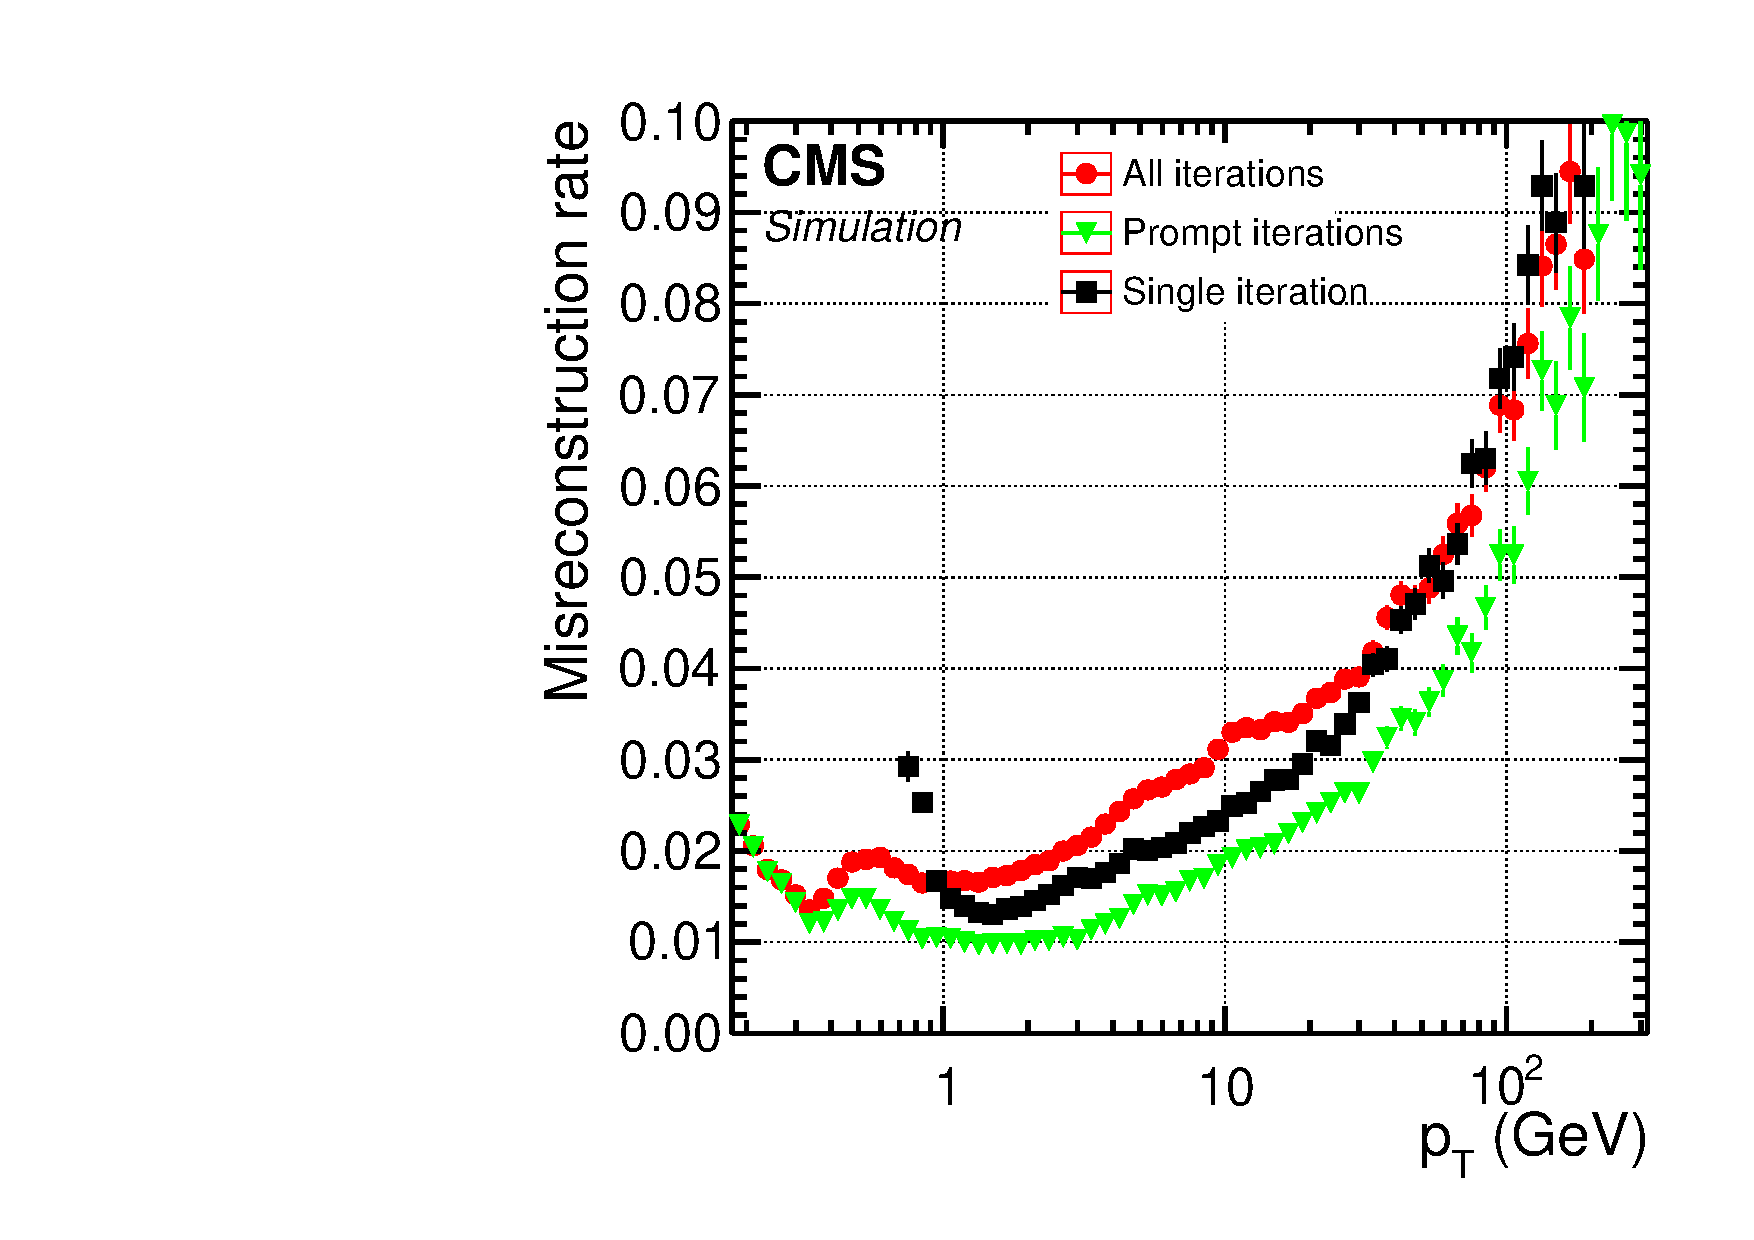
\includegraphics{SimReco/Figures/TrackingMis.pdf}}
\caption{Performance of the iterative tracking procedure \cite{Sirunyan:2017ulk}. The right figure shows the tracking efficiencies depending on the \pt of the charged particle for multiple different tracking approaches. 
         The left figure shows the rate to misreconstruct a track depending on the \pt of the charged particle for multiple different tracking approaches. Prompt iterations require at least one hit in the pixel detector.
  \label{fig:reco_trackingEff}}
  \end{center}
\end{figure}

The origins of the tracks along the beam axis are considered as primary vertices and sorted according to the \pt of the associated tracks.
The vertex with the highest \pt is assumed to be connected to the hard interaction. 
Additional vertices are caused by additional proton-proton collisions occuring in the same bunch crossing as the hard interaction.
This so-called pile-up leads to an average of 16 primary vertices in the 2016 dataset. In order to suppress the influence of pile-up tracks originating from
a pile-up, vertex are removed from the reconstruction. This applies to tracks within jets as well as other particles.

\section{Electron reconstruction}
\label{sec:SimReco_Ele}


The reconstruction of electrons is based on the combination of information from the tracker and the calorimeters.
Both electron and photon reconstruction require an ECAL cluster with a significant energy deposit.
For an electron, this cluster also contains the energy deposited by the bremsstrahlung photons.
The energy deposited in the HCAL region corresponding to the ECAL cluster is required to have less than 10\% of the energy deposited in the ECAL.
This requirement allows to separate electrons and photons from hadrons.
In order to be identified as an electron, a physics object needs a cluster of ECAL energy to be associated with a track.
In case no track is found, the physics object is identified as a photon.

The association between ECAL cluster and track is either seeded from both the tracker or from the ECAL.
The combination of both approaches increases reconstruction efficiency as shown in Figure \ref{fig:reco_eletrackseed}.
The main gain of efficiency applies to electrons with a $\pt$ below 10 $\GeV$, but even for electrons with higher \pt a few percent of efficiency are recovered.
Both the ECAL cluster and the track need to fulfill certain quality criteria applying to shower shape or track fitting.

\begin{figure}[htbp!]
  \begin{center}
      \resizebox{0.49 \textwidth}{!}{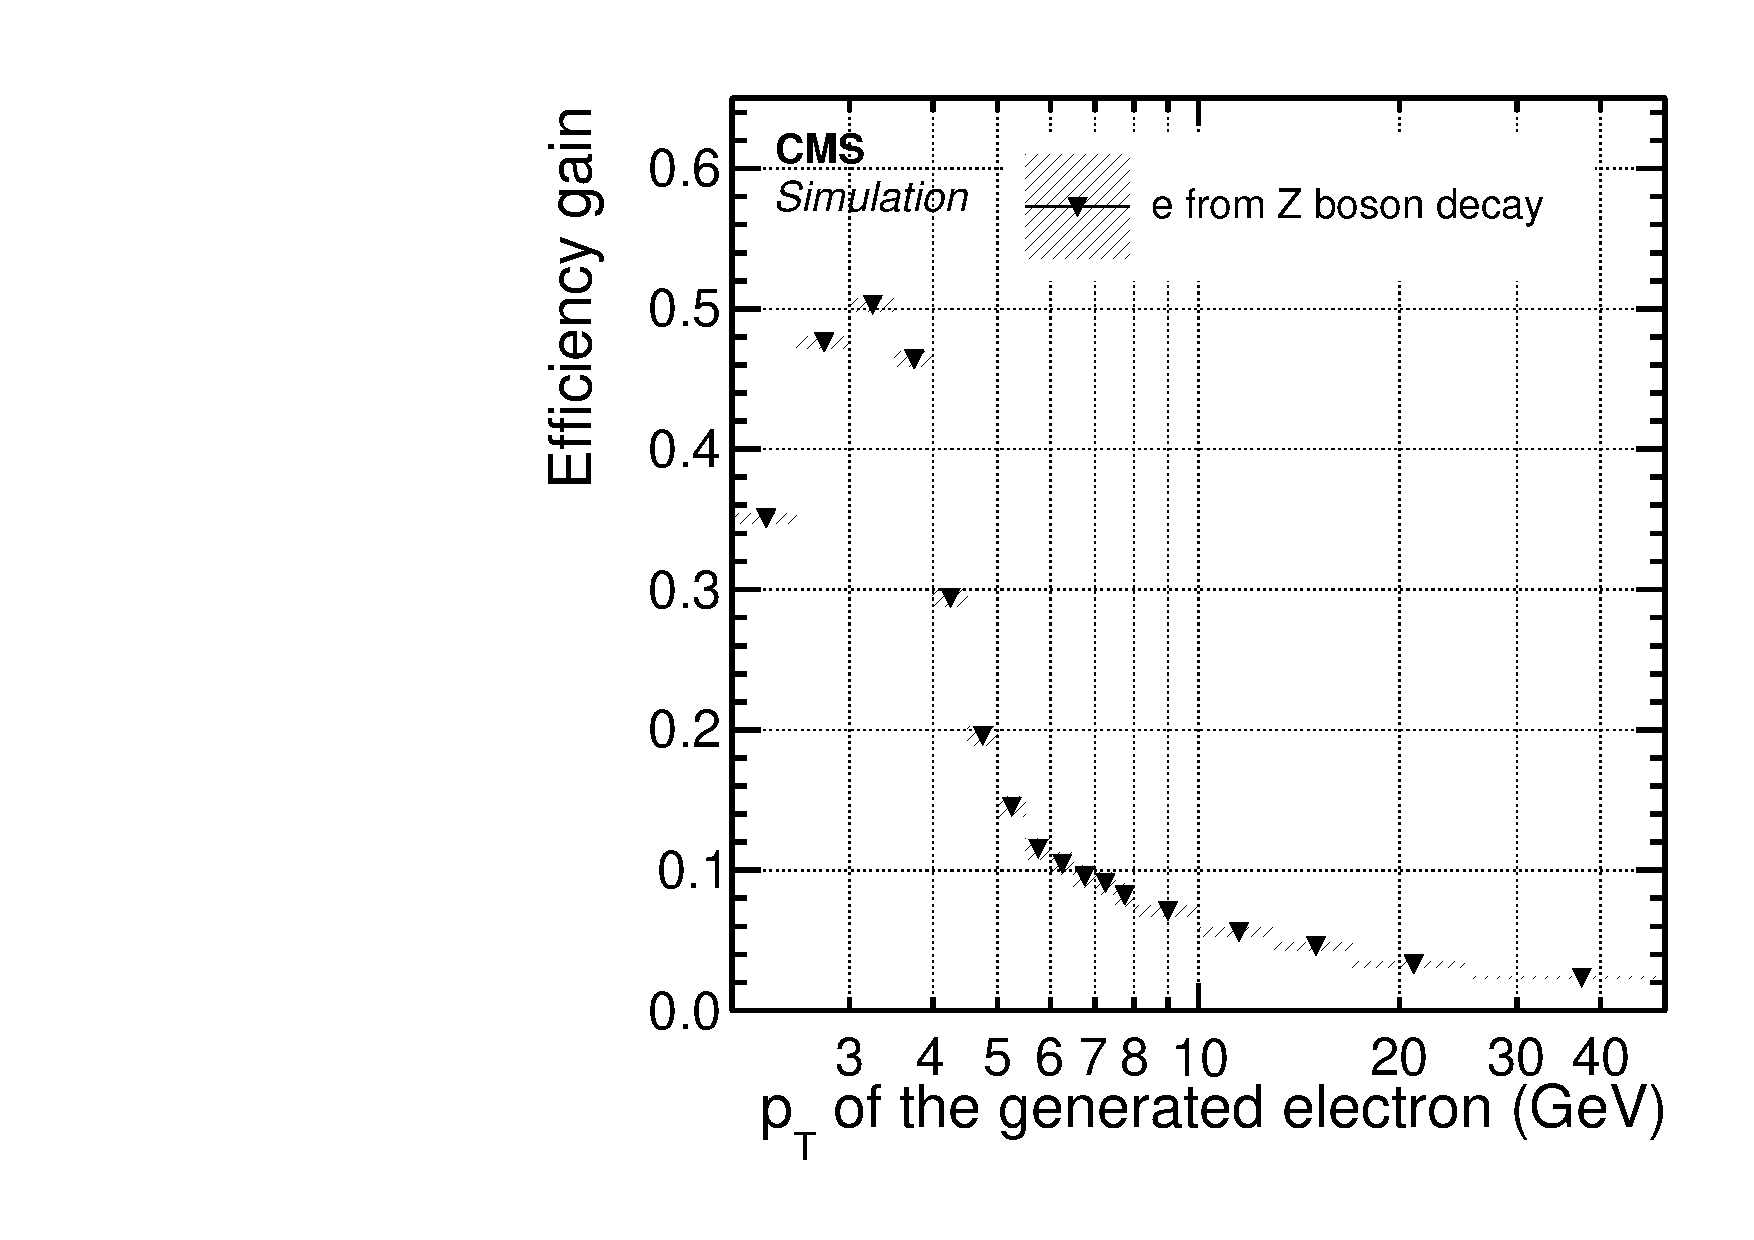
\includegraphics{SimReco/Figures/EleTrackSeed.pdf}}
\caption{Absolute gain in efficiency of the tracking in electrons when adding tracker-based seeding as a function of electron \pt\cite{Sirunyan:2017ulk}. 
         The efficiency is measured in simulated Z boson decays.
  \label{fig:reco_eletrackseed}}
  \end{center}
\end{figure}

Electrons also need to be isolated: The energy deposited in a cone around an electron is required to be below 6\% of the \pt of the electron.
The relative isolation is sensitive to contributions from pile-up. Contributions from charged particles that are not coming from the vertex of the hard collisions
are subtracted from the isolation. The pile-up contribution from non-charged particles is harder to determine. It is estimated according to the general energy density
in the event and subtracted from the isolation.
The combined efficiency to identify an electron is shown in Figure \ref{fig:reco_eleeff} as a function of the \pt and the $\eta$ of the electron.
It is measured with the Tag and Probe method, described in Section \ref{sec:TriggerTPMethod}.
As can be seen in Figure \ref{fig:reco_eleeff}, the efficiency depends more strongly on the $\pt$ of the electron than on its $\eta$ coordinate. 
The efficiency measured in data agrees with the one measured in simulation within $10\%$. 

\begin{figure}[htbp!]
  \begin{center}
      \resizebox{0.49 \textwidth}{!}{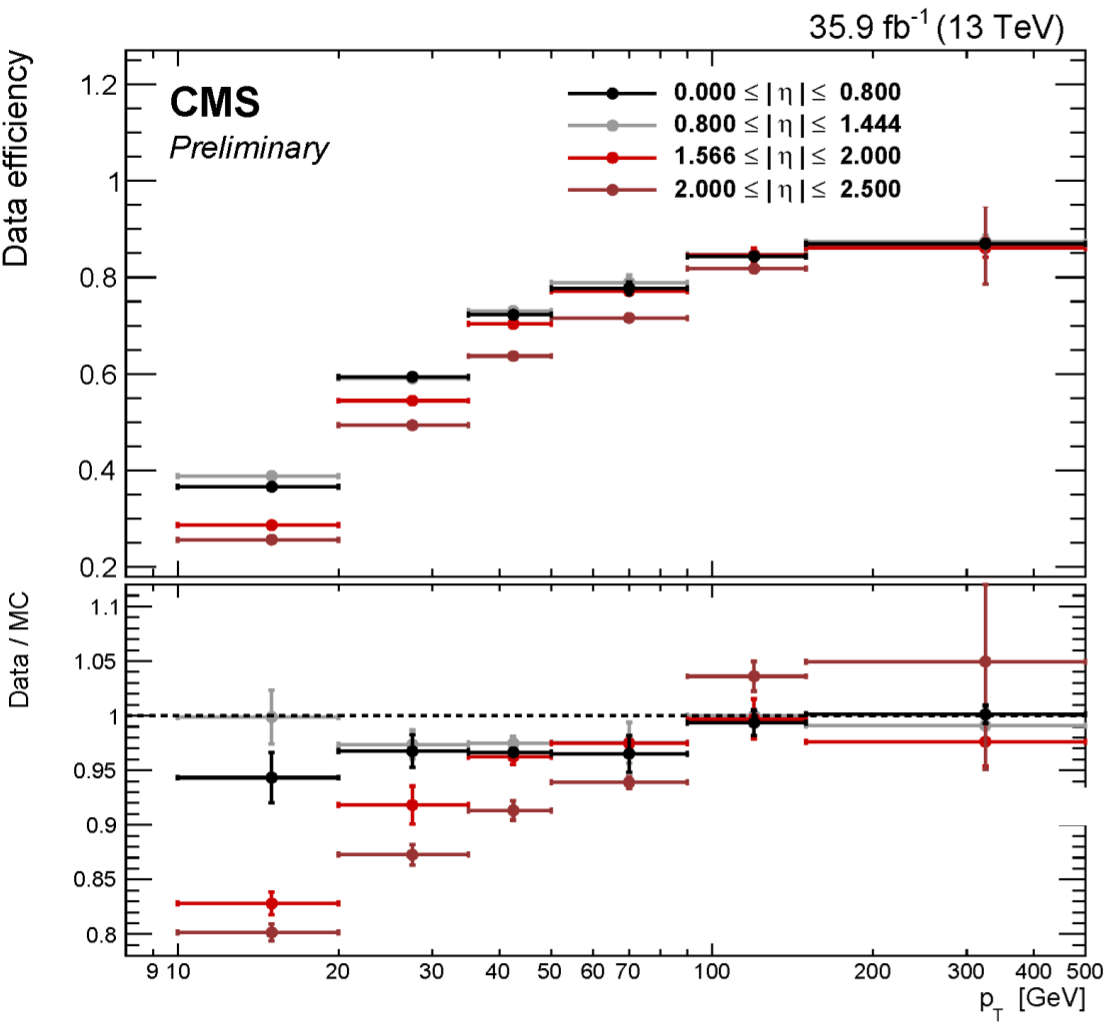
\includegraphics{SimReco/Figures/EleEff}}
\caption{Efficiency of the electron identification depending on the \pt and the $\eta$ of the electron\cite{CMS-DP-2017-004}.
         The upper panel shows the efficiency measured in data. The lower panel shows the efficiency in data divided by the efficiency in simulation. 
  \label{fig:reco_eleeff}}
  \end{center}
\end{figure}

The simulation is corrected according to the efficiency measurement in data. For each reconstructed electron, an $\eta$ and \pt dependent weight is assigned to each event,
so that the simulation is rescaled to match the data. The weight itself is calculated by dividing the efficiency in data by the efficiency in simulation: $w = \epsilon_{\mathrm{data}} (\pt,\eta) /\epsilon_{\mathrm{MC}} (\pt,\eta)$.
A correction of the same type is applied for the reconstruction of muons and the efficiency to trigger an event.

The electron energy is corrected to cover known biases from the electromagnetic calorimeter. Additionally, the energy resolution is found to be higher in simulation when compared to data.
Those biases are especially visible when comparing the Z boson mass peak in data and simulation \cite{CMS-DP-2016-026}.
Since the mass and width of the Z boson are extremely well known from LEP, and the behavior of these events in the detector is well understood, they allow for correcting the electron energy and resolution in simulation.

\section{Muon reconstruction}
\label{sec:SimReco_Mu}


Muons leave tracks in both the tracker and the muon system. The track in the muon system has to be matched to a track in the tracker to reconstruct a global muon.
The tracks need to be compatible with each other when propagated to a common surface.
Further quality requirements are applied to the inner track in the tracker.

Similar to the electrons, the muns are also required to be isolated. The energy in a cone around the muon (isolation) is required to be below 15\% of the muon \pt.
This energy is measured from charged particles coming from the primary vertex, neutral hadrons or photons. The impact of the pile-up on the neutral hadron and photon components
is estimated to be half of the contribution from charged pile-up and is subtracted from the total isolation.
The efficiency (measured with the Tag and Probe method, see Section \ref{sec:TriggerTPMethod}) for the identification and isolation requirements used in the analysis is shown in Figure \ref{fig:reco_mueff}.
The efficiency is above $90\%$ over nearly the whole range of $\eta$ and $\pt$.


\begin{figure}[htbp!]
  \begin{center}
      \resizebox{0.49 \textwidth}{!}{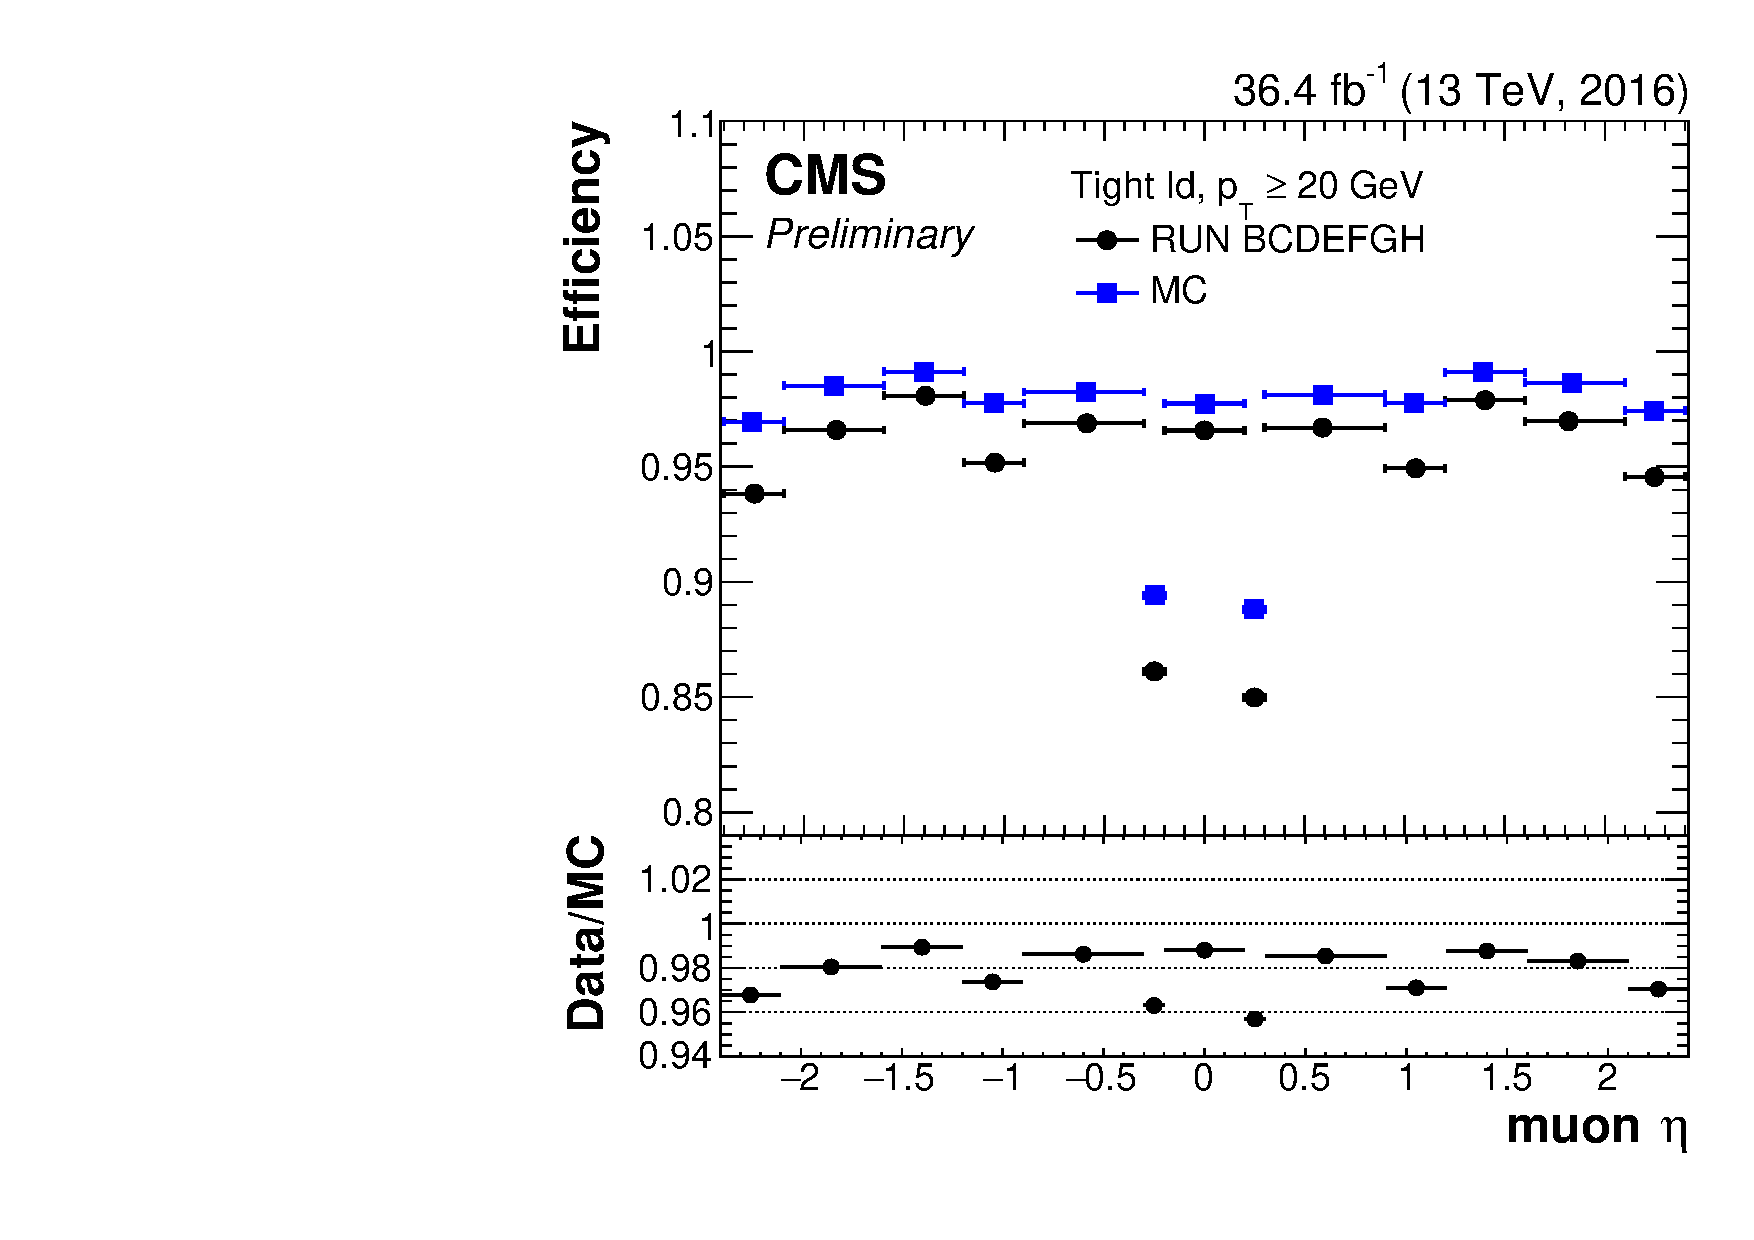
\includegraphics{SimReco/Figures/MuonIDEff}}
      \resizebox{0.49 \textwidth}{!}{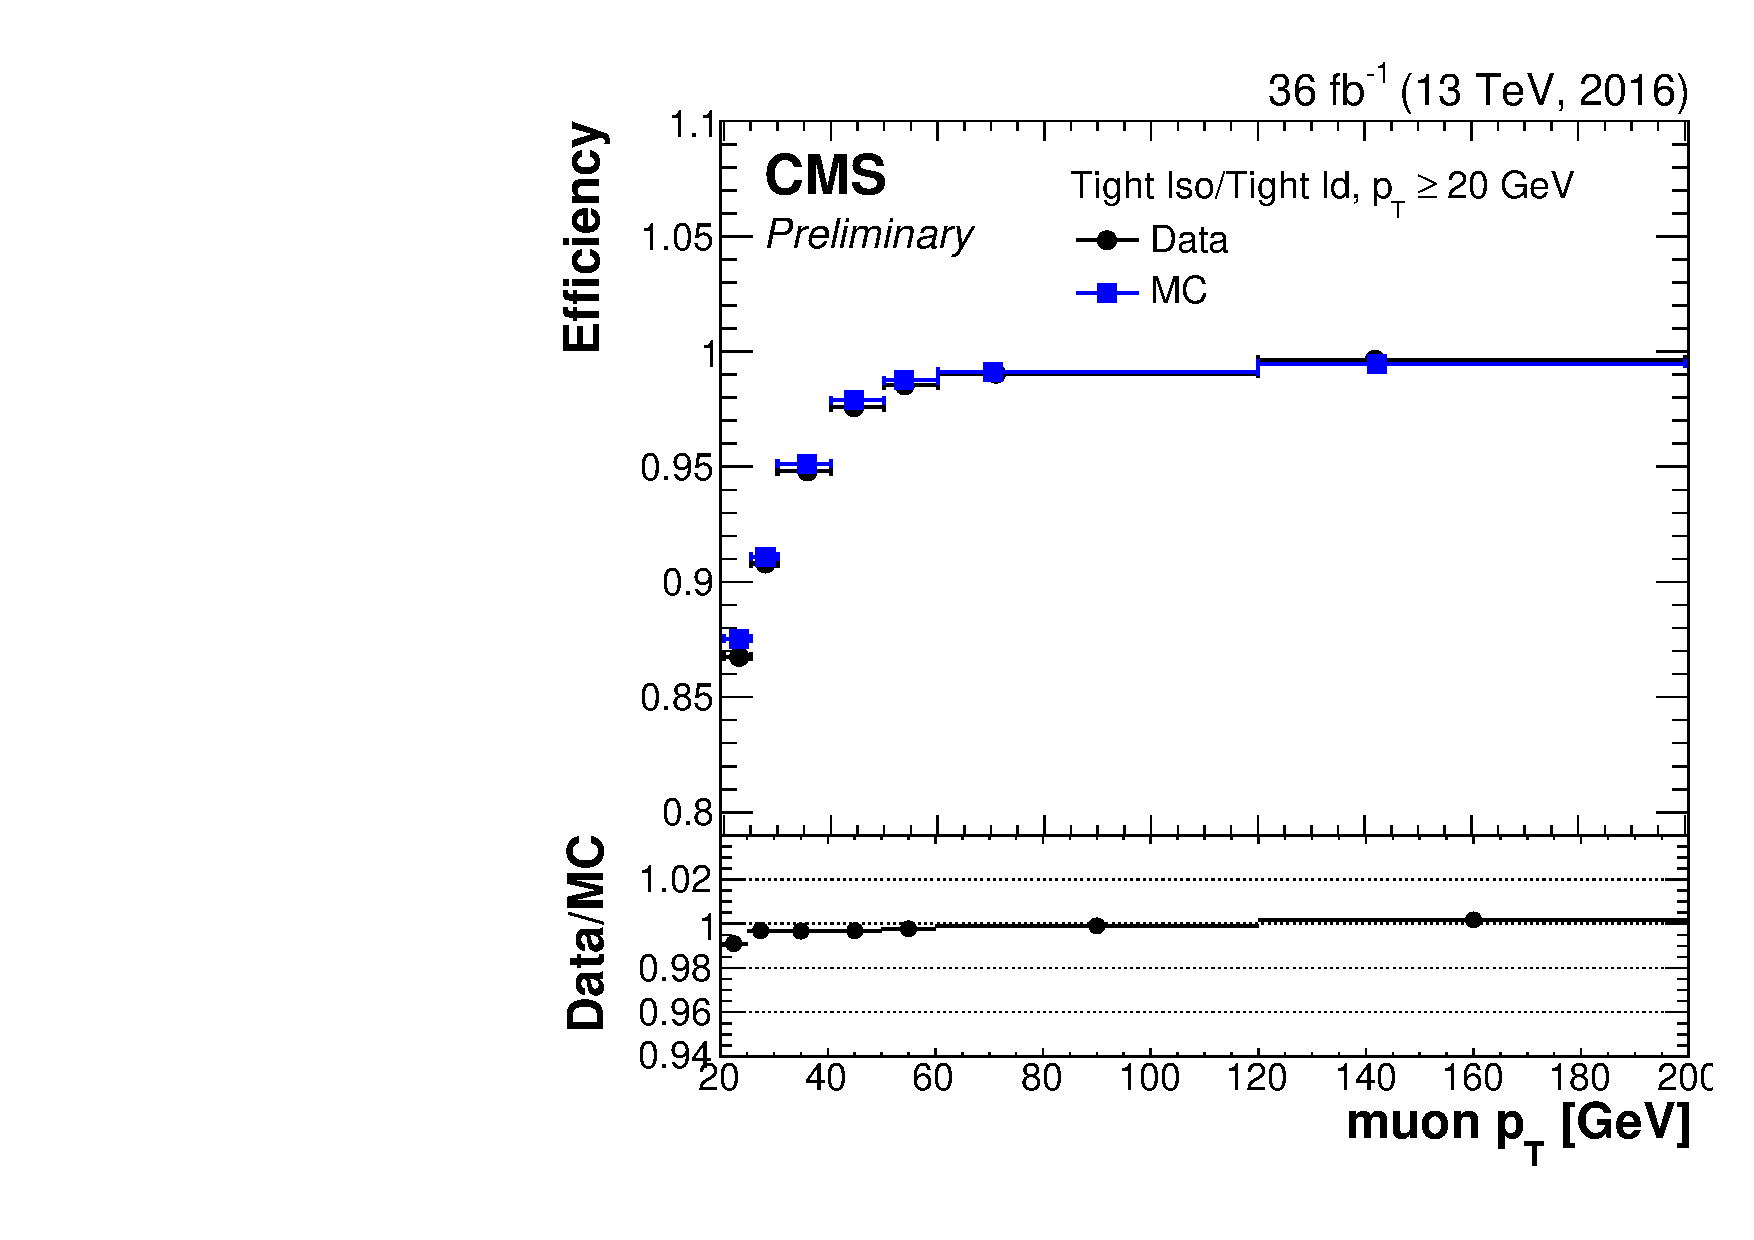
\includegraphics{SimReco/Figures/MuonIsoEff}}    
\caption{Efficiency of the identification (left) and isolation (right) for muons depending on $\eta$ (left) and $\pt$ right of the muon.
         The upper panels show the efficiency in data and simulation, while the lower panels show the ratio.
  \label{fig:reco_mueff}}
  \end{center}
\end{figure}

As described above for electrons, the small discrepancies of the simulation are corrected by event reweighting.

The resolution and scale of the \pt of the muons in data and simulation can be investigated by comparing the mass peak of the Z boson depending on the $\eta$ and $\phi$ of the two leptons.
Additionally, the forward and backward charge asymmetry is sensitive to differences between data and simulation.
The \pt of the muons is then corrected in simulation according to the disagreement observed. The corrections depend on the kinematics of the muon, its charge, the properties of the track of the muon and the simulated \pt
of the muon before the detector simulation.

\section{Reconstruction of jets}
\label{sec:SimReco_jetReco}

Jets are clustered from the individual particles reconstructed from the Particle Flow algorithm \cite{CMS-PAS-JME-16-003}.
The clustering uses the anti-\kt algorithm \cite{Cacciari:2008gp} as implemented in \FASTJET \cite{Cacciari:2011ma} with a distance parameter of $R = 0.4$.
The impact of pile-up is reduced by removing charged hadrons not originating from the primary vertex \cite{CMS-PAS-JME-14-001}.
Neutral particles originating from pile-up are taken into account by correcting the jet 4-momenta for each event based on the jet area \cite{1126-6708-2008-04-005,CACCIARI2008119}.

\begin{figure}[htbp!]
  \begin{center}
      \resizebox{0.99 \textwidth}{!}{
\includegraphics{SimReco/Figures/JECDiagram}}  
\caption{Illustration of the sequential jet energy scale corrections applied to measured data and simulation \cite{Khachatryan:2016kdb}. The flavor correction is not applied.
  \label{fig:reco_jec}}
  \end{center}
\end{figure}


The corrections for the jet energy scale are illustrated in Figure \ref{fig:reco_jec}. They are applied sequentially to both measured data and simulation \cite{Khachatryan:2016kdb,CMS-PAS-JME-16-003}.
The first step corrects for remaining contributions from pile-up, which are determined by comparing jets in simulated events with and without the simulation of additional pile-up collisions.
In data, an additional correction is derived from the Random Cone method in zero bias events, where the energy deposition in randomly distributed areas is measured \cite{1748-0221-6-11-P11002}. These areas (cones) have the same geometrical properties as the cones used for the jet clustering, which allows to measure the average pile-up contribution of a jet depending on $\eta$ and $\phi$. The correction is parametrized depending on the energy density in the event, the jet area and the kinematic
properties of the jet. The pile-up correction also depends on the data taking period.

In the next step, the reconstructed jet energy in the simulation is compared to the energy of a simulated jet before the detector simulation. Neutrinos are explicitly excluded, since they cannot be measured in the detector.
The correction depends on \pt and $\eta$ of the jets and is applied to both measured data and simulation.

The last correction is only applied to data (the flavor corrections shown in Figure \ref{fig:reco_jec} are not used). It corrects for remaining differences in the jet response between data and simulation, which are determined
from dijet events. The correction depends on the \pt and $\eta$ of the jets.

The different jet response in measured data and simulation is illustrated in Figure \ref{fig:reco_jetresponse} showing the response measured in events containing photons and jets, and Drell-Yan events.
It also shows the uncertainty of the jet energy scale corrections. The numbers shown here are derived only for a subset of the full dataset and do not correspond to the corrections used later in the measurement.

\begin{figure}[htbp!]
  \begin{center}
      \resizebox{0.49 \textwidth}{!}{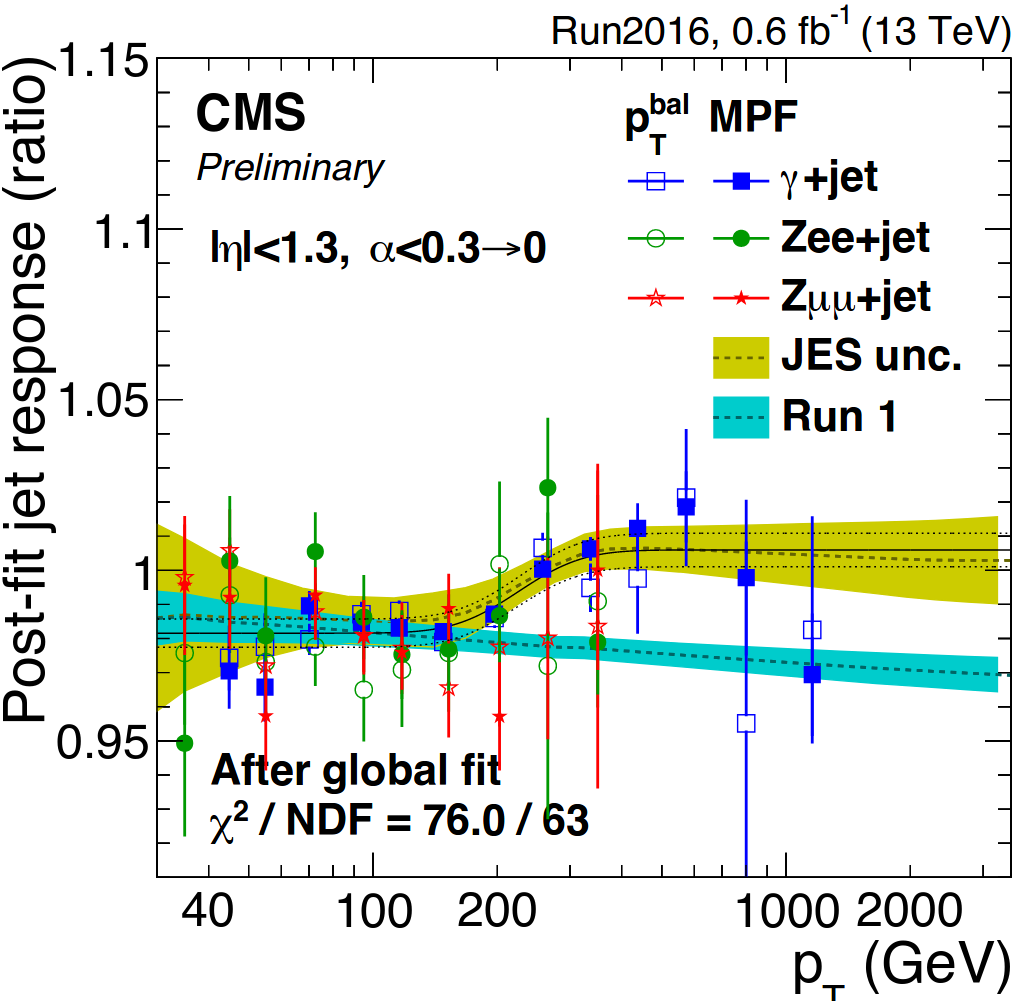
\includegraphics{SimReco/Figures/JetResponse}}  
\caption{The data to simulation ratio of the jet response measured in photon + jets and Z + jets events for a subset of data \cite{CMS-DP-2016-020}. The uncertainty for this dataset as well as the uncertainty for the dataset taken by the CMS collaboration
in Run 1 of the LHC are shown as colored bands. 
  \label{fig:reco_jetresponse}}
  \end{center}
\end{figure}


The jet energy resolution is determined from the width of the jet response function, defined as the ratio between the \pt of a simulated jet before and after reconstruction. It is found to be different in measured data and simulation. The \pt of the jets in simulation is rescaled depending on the simulation by the following
factor:

\begin{equation}
\mathrm{SF} = 1 + (\mathrm{SF}_{\mathrm{reso.}}-1) \frac{\pt - \pt^{gen}}{\pt}.
\end{equation}
Here, $\mathrm{SF}_{\mathrm{reso.}}$ denotes the resolution scale factor and $\pt^{gen}$ stands for the \pt of the simulated jet before the simulation of the detector response. 

If all particles from a collision are correctly reconstructed, the overall \pt of the events should be balanced, due to momentum conservation and the initial state particles not having momentum in the transverse direction.
Particles that cannot be reconstructed, such as neutrinos, lead to an imbalance in the overall measured transverse momentum. This quality is often referred to as missing transverse energy \ETmiss \cite{CMS-PAS-JME-16-004}.
The \ETmiss is reconstructed by a multivariate analysis using all other physics objects as well as unassociated energy deposits. It also takes the resolution of the other objects into account.
Since it is not used in the measurement, it is not described in further detail.

\section{Identification of b jets}
\label{sec:SimReco_BjetReco}


The large lifetime of the B hadron leads to a signature in which the decay vertex is often displaced from the original interaction.
These secondary vertices together with the displaced tracks and the properties of the jet itself are combined in the CSVv2 algorithm to identify jets originating from a b quark \cite{BTV16002}.
Sensitive variables are combined into a neural network which is trained against both jets originating from light jets as well as jets originating from c quarks.
The result is a single value (discriminator) with the cut chosen according to the desired efficiency and background rejection.

The tight working point chosen for this analysis has a very low rate of misidentifying a light jet as a b jet (mistag rate) with $\sim0.1\%$. The efficiency to correctly identify a jet from a b quark
as a b jet is measured to be $\sim40\%$ \cite{BTV16002}. These numbers are obtained for jets with an average transverse momentum of $\pt = 70\;\GeV$. A lower efficiency can be expected for b jets with a lower \pt.

The efficiency in simulation is corrected according to the efficiency measured in data. The difference measured in events containing both muons and jets and in \ttbar events is shown in Figure \ref{fig:reco_btagsf}.

\begin{figure}[htbp!]
  \begin{center}
      \resizebox{0.89 \textwidth}{!}{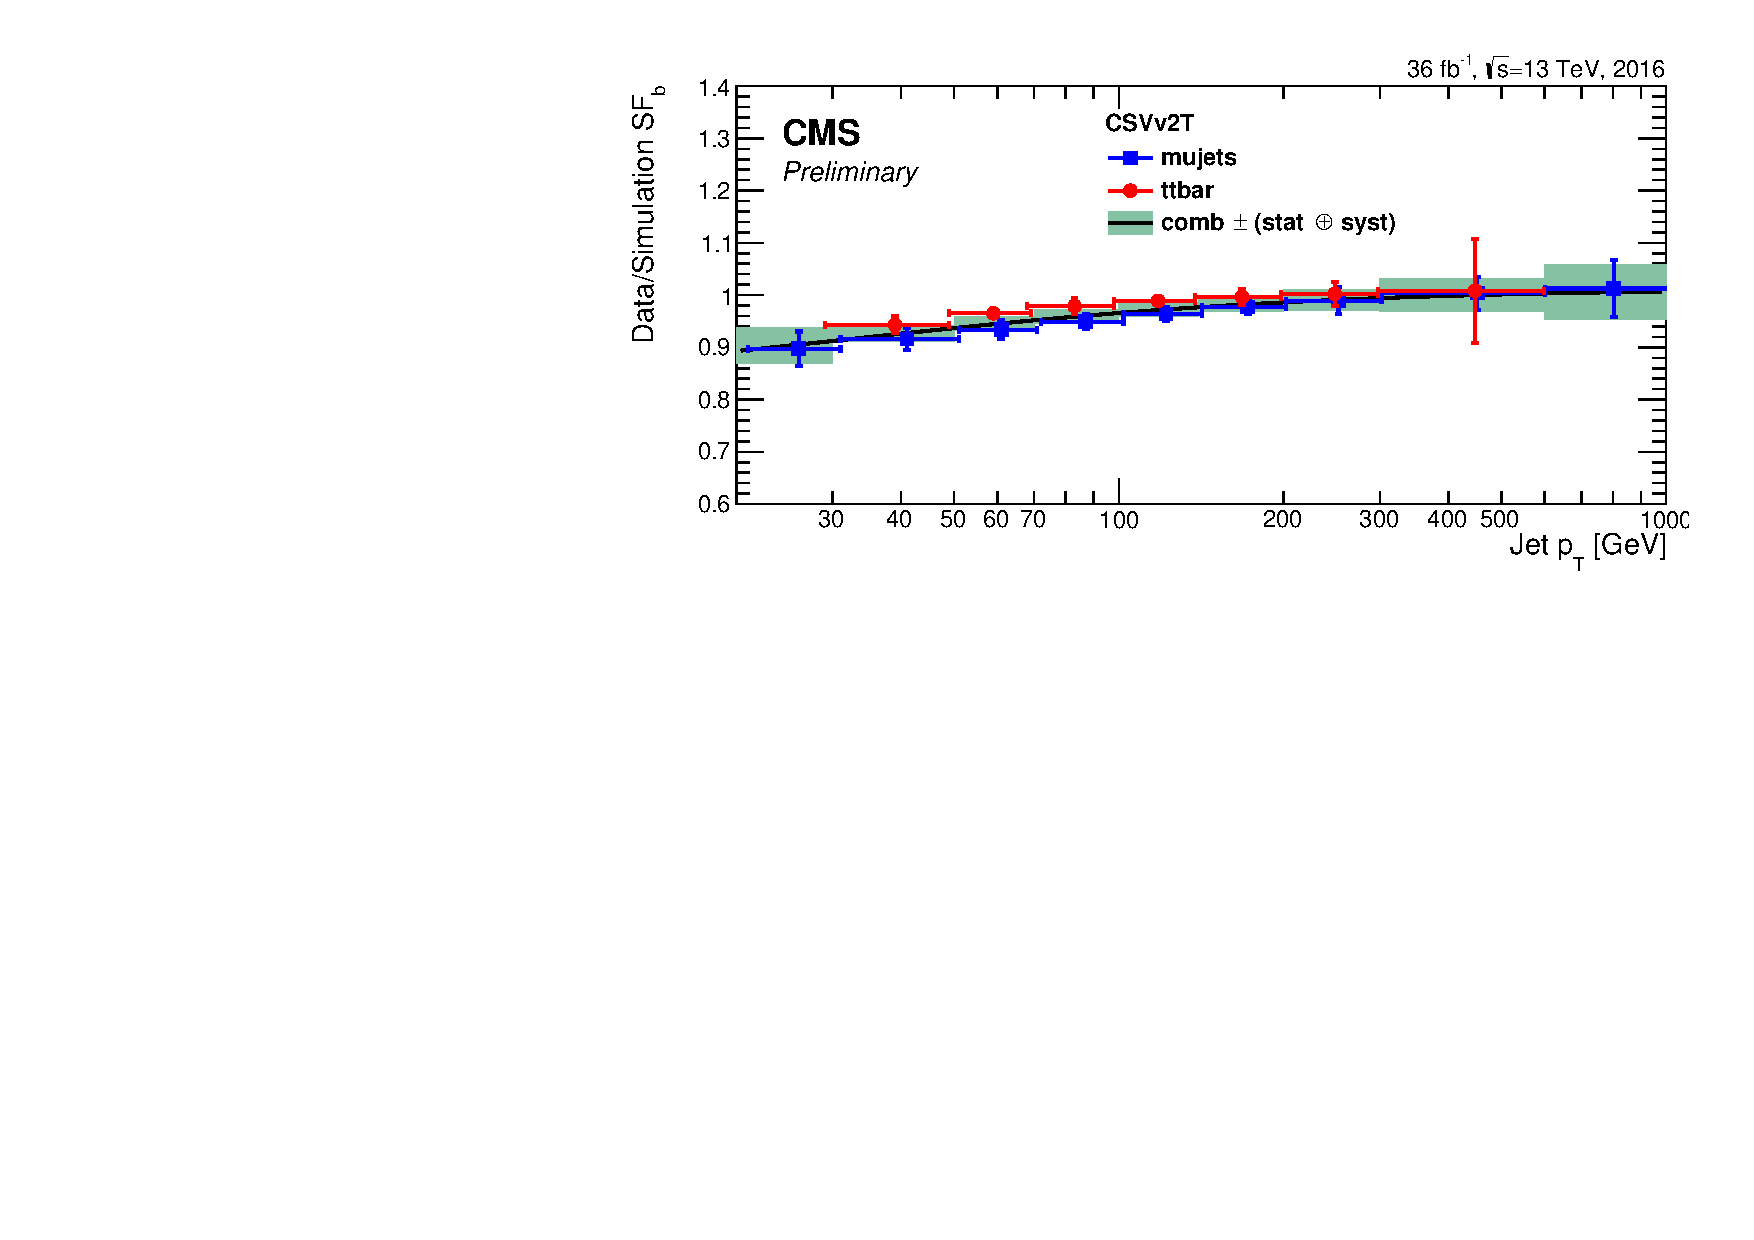
\includegraphics{SimReco/Figures/BTagSF}}  
\caption{Scale factor between the b jet identification efficiency measured in data and simulation. The measurement is performed with events containing jets and muons and in \ttbar events \cite{CMS-DP-2017-012}
  \label{fig:reco_btagsf}}
  \end{center}
\end{figure}

The difference between data and simulation is corrected by applying event weights. These event weights are not calculated directly from the scale factor but depend on the number of jets and the
efficiency to correctly identify a b jet in data as well as simulation.
The weights are calculated as the ratio of the probabilities to find b tagged jets in data and simulation:

\begin{eqnarray}
P(\mathrm{Data}) & = &\prod_{i=tagged} \epsilon_i^{data} \prod_{j=not tagged} (1-\epsilon_j^{Data}) \\
P(\mathrm{MC})& = &\prod_{i=tagged} \mathrm{SF}_i\epsilon_i^{MC} \prod_{j=not tagged} (1-\mathrm{SF}_j\epsilon_j^{MC}).
 %w = \frac{P(\mathrm{Data})}{P(\mathrm{MC})}.
\end{eqnarray}

Here, $\epsilon$ denotes the identification efficiency for a b jet in data and simulation respectively, while $\mathrm{SF}$ stands for the scale factor for that jet.
Both the efficiency and the scale factor depend on the kinematic properties of the jet.

